\documentclass[a4paper,12pt]{article}
\usepackage[french]{babel}
\usepackage[utf8]{inputenc}
\usepackage{graphicx}
\usepackage{amsmath, amssymb}
\usepackage{algorithm}
\usepackage{titlesec}
\usepackage{algpseudocode}
\usepackage{algcompatible}
\usepackage{hyperref}
\usepackage{listings}
\usepackage{xcolor}
\usepackage{caption}

\lstset{
    language=Python,
    basicstyle=\ttfamily\footnotesize,
    keywordstyle=\color{blue},
    commentstyle=\color{gray},
    stringstyle=\color{red},
    breaklines=true,
    frame=single
}

\usepackage[french]{babel}  % Langue du document
\usepackage[utf8]{inputenc}  % Encodage des caractères
\usepackage[T1]{fontenc}  % Meilleure gestion des accents
\usepackage{graphicx}  % Inclusion d'images
\usepackage{amsmath, amssymb}  % Mathématiques
\usepackage{hyperref}  % Liens hypertextes
\usepackage{listings}  % Affichage du code source
\usepackage{caption}
\usepackage{subcaption}
\usepackage{geometry}  % Mise en page
\geometry{left=2.5cm,right=2.5cm,top=2.5cm,bottom=2.5cm} 
\graphicspath{{images/}}

\title{Analyse d'identité d'auteurs et détection de plagiat}
\author{CHEDJARI EL MEUR Hadjer \\ NANMEDIGOU Yendoumban\\ Université de Caen Normandie}
\date{Mars 2025}

\begin{document}
\maketitle
\begin{abstract}
Ce rapport présente la conception et l'implémentation d'un système de détection de plagiat utilisant des techniques de tokenisation, de vectorisation (CountVectorizer, TF-IDF) et divers classificateurs (Naïve Bayes, Perceptron, etc.).
\end{abstract}

\tableofcontents

% Sections incluses depuis d'autres fichiers
\newpage
\section{Introduction}

Avec l’augmentation constante du volume de documents mis en ligne, le plagiat est devenu une problématique centrale dans de nombreux domaines, notamment en milieu académique et juridique. Identifier l’origine d’un document ou d’une partie de texte est un défi important pour assurer l’intégrité des contenus et lutter contre la fraude intellectuelle.

L’objectif de ce projet est de mettre en œuvre des techniques de traitement automatique du langage naturel (\textit{NLP}) afin d’analyser le contenu textuel et d’évaluer la similarité entre documents. Cette approche repose sur plusieurs étapes clés : la transformation des textes en représentations exploitables, l’implémentation de métriques de comparaison, et l’utilisation de modèles d’apprentissage automatique pour classer et regrouper les textes selon leur origine.

Dans ce cadre, nous avons choisi de développer notre propre pipeline de détection, sans recourir à des implémentations toutes faites. Cela inclut la création d’un tokenizer, la vectorisation des documents, ainsi que l’implémentation et l’évaluation de différents algorithmes de classification. Une analyse quantitative des résultats sera menée afin de comparer les performances des différentes approches et d’identifier les facteurs influençant leur efficacité.

Ce rapport détaille les choix méthodologiques adoptés, les techniques mises en œuvre et les résultats obtenus, dans le but de mieux comprendre les enjeux liés à la détection de plagiat et d’évaluer l’efficacité des différentes stratégies d’analyse.

\section{Objectifs du Projet}

Pour concevoir un système de détection de plagiat, nous avons défini plusieurs objectifs techniques et méthodologiques :

\subsection{Prétraitement et Extraction des Caractéristiques}
L’une des étapes clés du projet consiste à transformer un texte brut en une représentation exploitable par un algorithme de classification. Pour cela, nous avons :
\begin{itemize}
    \item[-] Développé un tokenizer capable de gérer la ponctuation, la casse, les stopwords et la lemmatisation.
    \item[-] Expérimenté différentes stratégies d’\textbf{n-grams} afin d’améliorer la capture des structures linguistiques.
    \item[-] Implémenté nos propres versions de \textbf{Bag-of-Words} et \textbf{TF-IDF}.
\end{itemize}

\subsection{Développement des Modèles de Classification}
Nous avons choisi d’implémenter plusieurs modèles afin de comparer leurs performances et d’identifier ceux les plus adaptés à notre problème. Nos implémentations incluent :
\begin{itemize}
    \item[-] \textbf{Naïve Bayes}, pour sa rapidité et son efficacité sur des données textuelles.
    \item[-] \textbf{Perceptron et Régression Logistique}, pour tester des approches linéaires d’apprentissage.
    \item[-] \textbf{Arbre de Décision, Random Forest et AdaBoost}, afin d’évaluer des approches non linéaires basées sur des ensembles de modèles.
\end{itemize}

\subsection{Optimisation et Expérimentations}
Une attention particulière a été portée à l’évaluation et à l’optimisation des modèles :
\begin{itemize}
    \item[-] Nous avons mis en place un \textbf{early stopping} pour éviter le sur-apprentissage et optimiser le temps d’entraînement.
    \item[-] Une évaluation détaillée des performances a été réalisée en utilisant les métriques \textbf{précision, rappel et F1-score}.
    \item[-] Nous avons analysé l'impact des hyperparamètres (taille des n-grams, régularisation, profondeur des arbres) sur les performances.
\end{itemize}

En suivant cette méthodologie, notre objectif est de construire une solution fiable et adaptable, tout en garantissant une compréhension approfondie des algorithmes sous-jacents.

\newpage
\section{Implémentation et Algorithmes}

\subsection{Tokenization}

La première étape du pipeline consiste à découper le texte en tokens. Nous avons appliqué :

\begin{algorithm}[H]
\caption{Tokenization}
\begin{algorithmic}[1]
\State \textbf{Entrée} : Texte brut $T$
\State \textbf{Sortie} : Liste de tokens $L$
\State Convertir $T$ en minuscules
\State Supprimer la ponctuation
\State Découper $T$ en mots (tokens)
\State Supprimer les stopwords de $T$
\State Appliquer la lemmatisation sur les tokens
\State \textbf{Retourner} $L$
\end{algorithmic}
\end{algorithm}
\textbf{Complexité :}  
La complexité de la tokenisation dépend du type d’approche utilisée :
\begin{itemize}
    \item Pour une tokenization basée sur des expressions régulières : 
    \begin{equation}
    O(n)
    \end{equation}
    où \( n \) est la longueur du texte.
    \item Pour une tokenization basée sur un dictionnaire avec recherche binaire :
    \begin{equation}
    O(n \log k)
    \end{equation}
    où \( k \) est la taille du dictionnaire.
\end{itemize}

\subsection{Extraction des caractéristiques} Cette étape transforme les tokens générés précédemment en représentations numériques exploitables par les algorithmes d'apprentissage automatique.

Nous avons utilisé deux méthodes :
\begin{itemize}
    \item \textbf{CountVectorizer} : Nombre d’occurrences de chaque mot
    \item \textbf{TF-IDF} : Importance relative des mots
\end{itemize}
Pour cela on distingue 2 parties principales:
\begin{itemize}
    \item[•] {Indexation} : Associe un index unique à chaque mot du vocabulaire.
    \item[•] {Représentation} : Génère une matrice où :
    \begin{itemize}
        \item[] Chaque ligne représente un document.
        \item[] Chaque colonne correspond à un mot du vocabulaire.
    \end{itemize}
\end{itemize}
\subsubsection{CountVectorizer}
CountVectorizer transforme un texte en une matrice de fréquences des mots.
\begin{algorithm}[H]
\caption{CountVectorizer}
\begin{algorithmic}[1]
\State \textbf{Entrée} : Liste de documents de test $D = \{d_1, d_2, \dots, d_N\}$
\State \textbf{Sortie} : Matrice de fréquence des termes $M$
\For{\textbf{chaque document} $d_i$}
    \For{\textbf{chaque mot} $w_j$ dans $d_i$}
        \State $M[i,j] \gets \text{nombre de fois que } w_j \text{ apparait dans } d_i$
    \EndFor
\EndFor
\State \textbf{Retourner} la matrice $M$
\end{algorithmic}
\end{algorithm}
\textbf{Complexité :}  
La transformation d’un corpus contenant \( n \) documents et \( m \) mots uniques dans le vocabulaire est :
\begin{equation}
O(n \cdot m)
\end{equation}
où :
\begin{itemize}
    \item \( n \) : nombre de documents.
    \item \( m \) : nombre total de mots uniques.
\end{itemize}

\subsubsection{TF-IDF}
Cette d’extraction de caractéristiques textuelles Pondère les mots en fonction de :
    \begin{itemize}
        \item[-] Leur fréquence dans un document.
        \item[-] Leur rareté dans l’ensemble du corpus.
    \end{itemize}
L’équation de TF-IDF est :

\[
\text{TF-IDF}(t,d) = \text{TF}(t,d) \times \log \frac{N}{\text{DF}(t)}
\]
où :
\begin{itemize}
    \item \( TF(t, d) \) : fréquence du terme \( t \) dans le document \( d \).
    \item \( f_t \) : nombre d’occurrences du terme \( t \) dans \( d \).
    \item \( N \) : nombre total de mots dans \( d \).
    \item \( IDF(t) \) : inverse de la fréquence du document.
    \item \( N_d \) : nombre total de documents.
    \item \( N_t \) : nombre de documents contenant le terme \( t \).
\end{itemize}
\begin{algorithm}[H]
\caption{Calcul de TF-IDF}
\begin{algorithmic}[1]
\State \textbf{Entrée} : Liste de documents $D = \{d_1, d_2, \dots, d_N\}$
\State \textbf{Sortie} : Matrice TF-IDF $M$
\For{\textbf{chaque document} $d_i$}
    \For{\textbf{chaque terme} $t_j$ dans $d_i$}
        \State $\text{TF}(t_j, d_i) \gets \frac{\text{nombre de fois que } t_j \text{ apparait dans } d_i}{\text{total des mots dans } d_i}$
        \State $\text{DF}(t_j) \gets \text{nombre de documents contenant } t_j$
        \State $\text{IDF}(t_j) \gets \log \left( \frac{N}{\text{DF}(t_j)} \right)$
        \State $M[i,j] \gets \text{TF}(t_j, d_i) \times \text{IDF}(t_j)$
    \EndFor
\EndFor
\State \textbf{Retourner} la matrice TF-IDF $M$
\end{algorithmic}
\end{algorithm}
\textbf{Complexité :}  
Le calcul du TF-IDF a une complexité de :
\begin{equation}
O(n \cdot m)
\end{equation}
où :
\begin{itemize}
    \item \( n \) : nombre de documents.
    \item \( m \) : nombre de mots uniques dans le corpus.
\end{itemize}

\subsection{Modéles de classification}
A ce niveau les matrices de caractéristiques sont Utilisées pour entraîner le classificateur et prédire si un document est un "plagiat" ou "non plagiat".

\subsubsection{Naïve Bayes}
\begin{equation}
P(y|X) = \frac{P(X|y) P(y)}{P(X)}
\end{equation}
où :
\begin{itemize}
    \item[-] \( P(y|X) \) : probabilité a posteriori de la classe \( y \) sachant les caractéristiques \( X \).
    \item[-] \( P(X|y) \) : probabilité d’observer \( X \) sachant que l’étiquette est \( y \).
    \item[-] \( P(y) \) : probabilité a priori de la classe \( y \).
    \item[-] \( P(X) \) : probabilité totale d’observer \( X \).
\end{itemize}
\begin{algorithm}[H]
\caption{Naïve Bayes pour classification}
\begin{algorithmic}[1]
\State \textbf{Entrée} : Ensemble de données d'entraînement $\{(x_i, y_i)\}$, où $x_i$ est un vecteur de caractéristiques et $y_i$ est la classe
\State \textbf{Sortie} : Modèle de classification
\For{\textbf{chaque} classe $y$}
    \State Calculer la probabilité a priori $\hat{P}(y) = \frac{\text{nombre de } y \text{ dans les données d'entraînement}}{N}$
\EndFor
\For{\textbf{chaque} caractéristique $x_j$}
    \State Estimer la probabilité conditionnelle $\hat{P}(x_j | y)$ en utilisant les données d'entraînement
\EndFor
\State \textbf{Retourner} le modèle avec $\hat{P}(y)$ et $\hat{P}(x_j | y)$
\end{algorithmic}
\end{algorithm}
\textbf{Complexité :}  
L'entraînement de Naïve Bayes consiste à calculer les probabilités conditionnelles pour chaque attribut et chaque classe.  
\begin{equation}
O(n \cdot m)
\end{equation}
où :
\begin{itemize}
    \item \( n \) : nombre d'échantillons dans l'ensemble d'entraînement.
    \item \( m \) : nombre de caractéristiques (features).
\end{itemize}
La classification d’un nouvel échantillon se fait en :
\begin{equation}
O(m \cdot k)
\end{equation}
où \( k \) est le nombre de classes.

\subsubsection{Logistic Regression}
\begin{equation}
P(y=1|X) = \frac{1}{1 + e^{-(wX + b)}}
\end{equation}
où :
\begin{itemize}
    \item[-] \( P(y=1|X) \) : probabilité que \( X \) appartienne à la classe \( y=1 \).
    \item[-] \( w \) : vecteur des poids associés aux caractéristiques.
    \item[-] \( X \) : vecteur des caractéristiques de l'instance.
    \item[-] \( b \) : biais du modèle.
    \item[-] \( e \) : base du logarithme naturel (\(\approx 2.718\)).
\end{itemize}
\begin{figure}[H]
            \centering
            \begin{subfigure}[b]{0.4\textwidth}
                \centering
                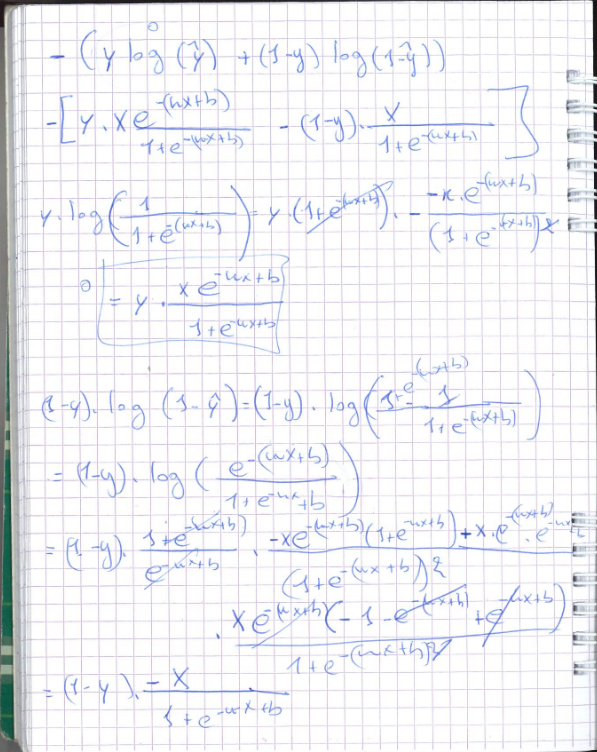
\includegraphics[width=\textwidth]{LR_db1.png}
                \caption{Original Image}
                \label{fig:original}
            \end{subfigure}
            \begin{subfigure}[b]{0.4\textwidth}
                \centering
                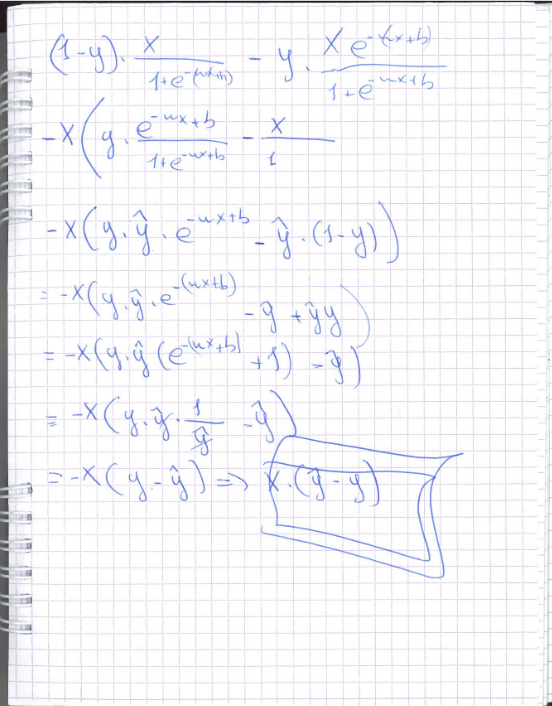
\includegraphics[width=\textwidth]{LR_dw2.png}
                \caption{After Histogram Normalization}
                \label{fig:original}
            \end{subfigure}
            \caption{ Calcule de Dw }
            \label{fig:cam_man_hn}
\end{figure}
\begin{figure}[H]
            \centering
            \begin{subfigure}[b]{0.4\textwidth}
                \centering
                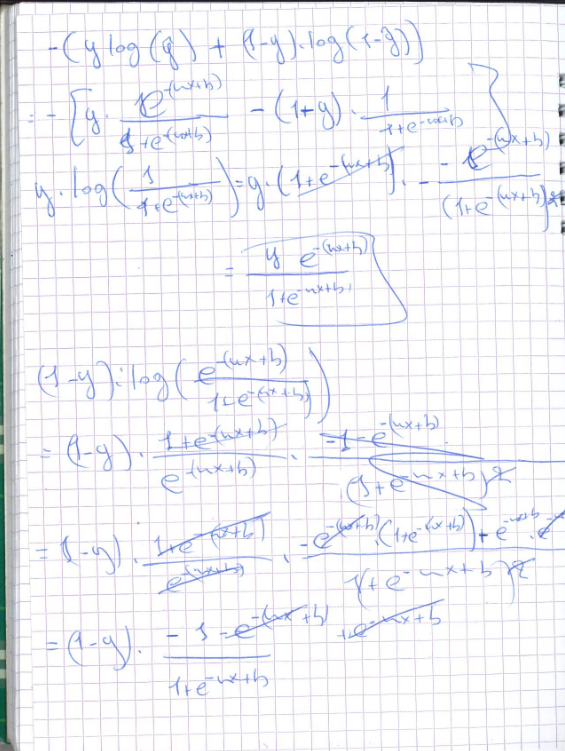
\includegraphics[width=\textwidth]{LR_dw1.png}
                \caption{Original Image}
                \label{fig:original}
            \end{subfigure}
            \begin{subfigure}[b]{0.4\textwidth}
                \centering
                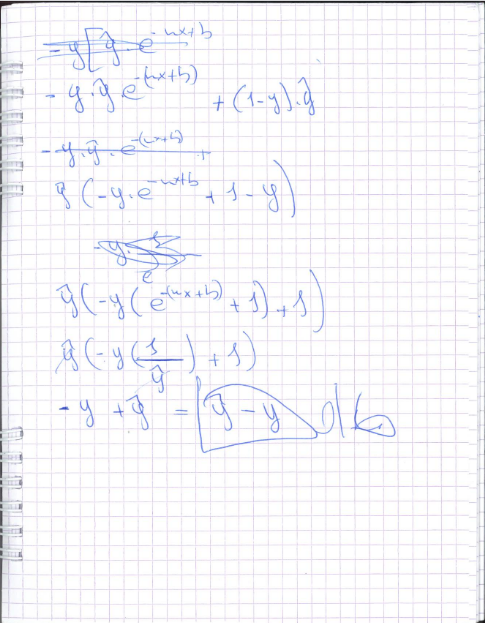
\includegraphics[width=\textwidth]{LR_db2.png}
                \caption{After Histogram Normalization}
                \label{fig:original}
            \end{subfigure}
            \caption{ Calcule de Db }
            \label{fig:cam_man_hn}
\end{figure}
\begin{algorithm}[H]
\caption{Régression Logistique pour classification}
\begin{algorithmic}[1]
\State \textbf{Entrée} : Ensemble de données d'entraînement $\{(x_i, y_i)\}$, où $x_i$ est un vecteur de caractéristiques et $y_i$ est la classe
\State Initialiser les poids $w$ et le biais $b$
\For{\textbf{chaque} échantillon $(x_i, y_i)$}
    \State Calculer la probabilité $\hat{y_i} = \sigma(w \cdot x_i + b)$, où $\sigma(z) = \frac{1}{1 + e^{-z}}$
    \State Calculer l'erreur $L = y_i \log(\hat{y_i}) + (1 - y_i) \log(1 - \hat{y_i})$
    \State Mettre à jour les poids $w$ et $b$ avec la descente de gradient :
    \State $w = w - \eta \frac{\partial L}{\partial w}$
    \State $b = b - \eta \frac{\partial L}{\partial b}$
\EndFor
\State \textbf{Retourner} $w, b$
\end{algorithmic}
\end{algorithm}
\textbf{Complexité :}  
L'entraînement est effectué via la descente de gradient, qui prend :
\begin{equation}
O(i \cdot n \cdot m)
\end{equation}
où :
\begin{itemize}
    \item \( i \) : nombre d'itérations.
    \item \( n \) : nombre d'échantillons.
    \item \( m \) : nombre de caractéristiques.
\end{itemize}
La classification d’un nouvel échantillon se fait en :
\begin{equation}
O(m)
\end{equation}

\subsubsection{Perceptron}
\begin{equation}
y = \text{sign}(wX + b)
\end{equation}
où :
\begin{itemize}
    \item \( y \) : classe prédite (\(+1\) ou \(-1\)).
    \item \( \text{sign}(z) \) : fonction qui retourne \( +1 \) si \( z \) est positif, sinon \( -1 \).
    \item \( w \) : vecteur des poids.
    \item \( X \) : vecteur des caractéristiques.
    \item \( b \) : biais.
\end{itemize}

\begin{figure}[H]
    \centering
    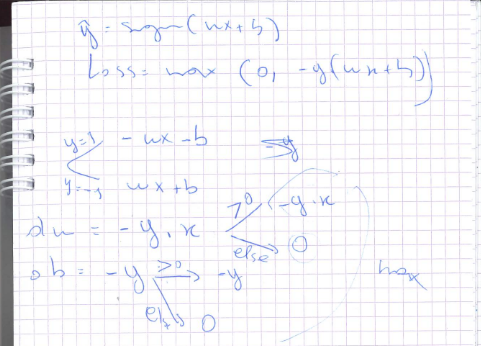
\includegraphics[width=0.5\linewidth]{perceptron.png}
    \caption{Calcule de Decent Gradient}
    \label{fig:mon_image}
\end{figure}

\begin{algorithm}[H]
\caption{Perceptron pour classification binaire}
\begin{algorithmic}[1]
\State \textbf{Initialisation} : poids $w$, biais $b$, taux d'apprentissage $\eta$
\For{\textbf{chaque} échantillon $(x_i, y_i)$}
    \State $\hat{y} = \text{sign}(w \cdot x_i + b)$
    \If{$\hat{y} \neq y_i$}
        \State $w = w + \eta (y_i x_i)$
        \State $b = b + \eta y_i$
    \EndIf
\EndFor
\State \textbf{Retourner} $w, b$
\end{algorithmic}
\end{algorithm}

\textbf{Complexité :}  
L'algorithme du perceptron apprend en ajustant les poids en fonction des erreurs. Sa complexité d'entraînement est :
\begin{equation}
O(i \cdot n \cdot m)
\end{equation}
et la classification d’un nouvel échantillon se fait en :
\begin{equation}
O(m)
\end{equation}

\subsubsection{Decision Tree}
\paragraph{Indice de Gini}
\begin{equation}
Gini = 1 - \sum p_i^2
\end{equation}
où :
\begin{itemize}
    \item[-] \( Gini \) : mesure d'impureté du nœud.
    \item[-] \( p_i \) : proportion d’éléments appartenant à la classe \( i \) dans le nœud.
\end{itemize}

\paragraph{Entropie}
\begin{equation}
Entropy = -\sum p_i \log_2 p_i
\end{equation}
où :
\begin{itemize}
    \item[-] \( Entropy \) : mesure d’incertitude dans la répartition des classes.
    \item[-] \( p_i \) : proportion d’éléments de la classe \( i \) dans le nœud.
    \item[-] \( \log_2 \) : logarithme en base 2.
\end{itemize}
\begin{algorithm}[H]
\caption{Arbre de Décision pour classification}
\begin{algorithmic}[1]
\State \textbf{Entrée} : Ensemble de données d'entraînement $\{(x_i, y_i)\}$, où $x_i$ est un vecteur de caractéristiques et $y_i$ est la classe
\State \textbf{Sortie} : Arbre de décision
\State Construire l'arbre récursivement :
    \For{\textbf{chaque} noeud de l'arbre}
        \State Calculer l'impureté (par exemple, entropie ou Gini) pour chaque caractéristique
        \State Choisir la caractéristique qui minimise l'impureté (meilleure séparation)
        \State Diviser l'ensemble de données en fonction de la caractéristique choisie
        \State Si le noeud est pur (impureté = 0) ou si un critère d'arrêt est atteint, arrêter
    \EndFor
\State \textbf{Retourner} l'arbre construit
\end{algorithmic}
\end{algorithm}
\textbf{Complexité :}  
L'entraînement d'un arbre de décision nécessite la recherche du meilleur attribut pour la division des données à chaque nœud. Cette opération a une complexité :
\begin{equation}
O(n \cdot m \log n)
\end{equation}
La classification d’un nouvel échantillon prend :
\begin{equation}
O(d)
\end{equation}
où \( d \) est la profondeur de l’arbre.



\subsubsection{Bagging (Bootstrap Aggregating)}

Bagging est une méthode d'ensemble qui vise à réduire la variance des modèles d'apprentissage supervisé. Il repose sur la création de plusieurs sous-échantillons des données d'entraînement en effectuant un \textbf{bootstrap sampling} (tirage avec remise). Chaque modèle est entraîné indépendamment sur un sous-échantillon et leurs prédictions sont ensuite combinées pour obtenir un modèle plus robuste. Le RandomForest en est une extension (un Bagging sur des arbres de décision).

\paragraph{Algorithme de Bagging}

\begin{algorithm}[H]
\caption{Algorithme de Bagging}
\begin{algorithmic}[1]
\State \textbf{Entrée} : Ensemble d'entraînement \( D \) de taille \( N \), Nombre de modèles \( M \), Modèle de base \( h \)
\For{$t = 1$ \textbf{to} $M$}
    \State Générer un échantillon \( D_t \) en tirant \( N \) instances de \( D \) avec remise.
    \State Entraîner un modèle \( h_t \) sur \( D_t \)
\EndFor
\State \textbf{Prédiction} :
\If{Classification}
    \State Retourner la majorité des prédictions des \( M \) modèles : \( \text{majorité}(h_1(x), h_2(x), ..., h_M(x)) \)
\Else
    \State Retourner la moyenne des prédictions des \( M \) modèles : \( \frac{1}{M} \sum_{t=1}^{M} h_t(x) \)
\EndIf
\end{algorithmic}
\end{algorithm}


\subsubsection{AdaBoost (Adaptive Boosting)}

AdaBoost est une technique de \textbf{boosting} qui combine plusieurs classificateurs faibles pour créer un modèle robuste. Contrairement au bagging, AdaBoost entraîne les modèles \textbf{séquentiellement} en pondérant les erreurs : les exemples mal classés reçoivent un poids plus important à chaque itération pour forcer le modèle suivant à mieux les apprendre.

\paragraph{Algorithme d'AdaBoost}

\begin{algorithm}[H]
\caption{Algorithme d'AdaBoost}
\begin{algorithmic}[1]
\State \textbf{Entrée} : Ensemble d'entraînement \( D = \{(x_1, y_1), ..., (x_N, y_N)\} \), Nombre de modèles \( M \), Modèle faible \( h \), Poids initialisés uniformément : \( w_i = \frac{1}{N} \)
\For{$t = 1$ \textbf{to} $M$}
    \State Entraîner un classificateur \( h_t \) sur les données pondérées \( (D, w) \)
    \State Calculer l'erreur pondérée \( e_t = \sum_{i=1}^{N} w_i \cdot \mathbb{1}(h_t(x_i) \neq y_i) \)
    \State Calculer le poids du modèle \( \alpha_t = \frac{1}{2} \ln \left(\frac{1 - e_t}{e_t}\right) \)
    \State Mettre à jour les poids des échantillons :
    \[
    w_i \leftarrow w_i \cdot e^{-\alpha_t y_i h_t(x_i)}
    \]
    \State Normaliser les poids \( w_i \) pour que \( \sum w_i = 1 \)
\EndFor
\State \textbf{Prédiction} : 
\State Prédire la classe pour un nouvel exemple \( x \) : 

H(x) = \text{sign} \left( \sum_{t=1}^{M} \alpha_t h_t(x) \right)
\end{algorithmic}
\end{algorithm}

\newpage
\section{Architecture}

\subsection{Paquetage}

Répondre aux objecttifs de notre projet a nécessité d'organiser notre travail en plusieurs packages et sous packages, chacun ayant un rôle bien défini.

\begin{figure}[H]
    \includegraphics[width=\textwidth]{rapport/images/paquetage.png}
\caption{Paquetage}
\end{figure}
\begin{figure}[H]
    \includegraphics[width=\textwidth]{rapport/images/classes_diag.png}
\caption{Diagramme de classes}
\end{figure}

\subsubsection{model} 
C'est le package central du fait qu'il contient toute la logique métier du détecteur de plagiat implémenté, des pré-processeurs de texte aux classifiers. Il est lui-même composé de 4 sous packages.

\paragraph{preprocessors}  
Les outils nécessaire au pré-traitement de texte, notamment le Tokenizer et le lemmatizer, sont contenu dans ce package.  
Le Tokenizer a pour fonction la première étape de notre chaîne de traitement. À partir d'un texte brut, quel sont les élements (mots ou sac de mots) que nous jugeons pertinents pour une extraction de caractéristiques. Pour cela, il dispose de la méthode \texttt{tokenize} qui prend en entrée le texte à tokenizer. Son attribut \texttt{stop\_words} (qui est initialisé par défaut aux stopwords anglais du module \texttt{nltk}), nous permettra de préciser quels mots ne sont pas nécessaires pour l'étape suivante. Quant à son \texttt{lemmatizer} (une fonction, initialisée à \texttt{None}), il nous permettra d'appliquer ou pas d'appliquer la lemmatization aux mots du texte traité.  
Notre lemmatizer est la fonction \texttt{lemmatize} du fichier \texttt{lemmatizer.py} qui prend en entrée une liste de mots et renvoie leur formes canoniques. Elle utilise pour cela le module \texttt{spacy}.

\paragraph{featurizers}  
Après la tokenization, l'extraction des caractéristiques sur les tokens générés est assurée par les featurizers, contenus dans ce package. Leur modèle est établi par la classe abstraite \texttt{Featurizer}. Un featurizer stocke le vocabulaire qu'il a appris, pour le réutiliser lors de l'extraction de traits, et dispose d'un tokenizer pour s'assurer que les éléments traités soient des tokens ; d'où ses attributs \texttt{vocabulary} et \texttt{tokenizer}. \texttt{n\_grams} est son attribut qui nous permettra de préciser les tailles des mots de sacs voulus. Quant aux méthodes, on peut lui faire apprendre du vocabulaire en lui donnant une liste de textes (méthode \texttt{fit}) et lui demander d'extraire les caractéristiques correspondant à une liste de textes (méthode \texttt{transform}). Sa méthode \texttt{fit\_transform} combine les deux étapes mentionnées précédemment. Les classes et \texttt{CountVectorFeaturizer} et \texttt{TfidfFeaturizer} sont les deux featurizers implémentés.

\paragraph{classifiers}  
C'est la prochaine étape, classification des textes (en réalité des caractéristiques extraites), qu'assure cet package. Un classifier, dont le modèle est défini par la classe abstraite \texttt{Classifier} peut être entraîné sur un ensemble de textes. C'est le rôle de sa méthode \texttt{fit}. Pour cela, on lui fournit la matrice de features où chaque ligne représente les caractéristique d'un texte, puis les classes auxqueles appartiennent ces textes. On pourra ensuite lui demander de déterminer la classe d'un ensemble de textes (méthode \texttt{predict}) en lui fournissant les matrices de features. Il stocke par ailleurs dans un attribut \texttt{classes} les classes rencontrées lors de son entraînement.

\paragraph{pipeline}  
Ce package contient notre détecteur de plagiat (classe \texttt{PlagiarismDetector}) qui met en place la chaîne de traitement du modèle de détection, du texte brut au résultat plagiat/pas plagiat. Ce détecteur est constitué d'un tokenizer, d'un featurizer et d'un classifier. Ces sont ses attributs. Il dispose de la méthode \texttt{train} pour s'entraîner sur des textes (cela consistera en l'entraînement, \texttt{fit}, de son featurizer et de sont classifier) et de la méthode \texttt{classify} pour déterminer si un texte est plagié ou pas.

\subsubsection{experiments}  
Les expérimentations réalisées sur notre modèles et les outils développés pour la cause, notamment le manager d'experimentations (\texttt{ExperimentManager}), l'évaluateur des métriques (\texttt{Metrics}) se trouvent dans ce package. \texttt{Metrics} dispose de méthodes statiques permettant d'évaluer l'accuracy, la précision, le rappel, la balanced accuracy et le score f1 d'un modèle. \texttt{ExperimentsManager} permettra lui de lancer les expériences sur les modèles évalués et les données qui lui ont été fournis. Le fichier \texttt{experiments.py} contient les expérimentations à proprement parler.

\subsubsection{gui}  
C'est le package dédié à la construction de notre interface graphique. Elle est conçue selon l'architecture MVC.

\subsubsection{util}  
Nous avons nécessiter des utilitaires qu'il a fallu nous même définir. Elles sont contenues dans le fichier \texttt{util.py}, seul fichier du package. Il s'agit entre autres de lecture de fichier ou de dossier (\texttt{read\_file} et \texttt{read\_files}) et de la partition d'ensemble (\texttt{partition}).

\subsubsection{tests}  
Des tests unitaires ont été réalisés sur les éléments non triviaux de notre modèle, notamment la tokenization et la featurization.

\subsection{Chaîne de traitement}  
La description du paquetage ci-dessus dessine déjà la chaîne de traitement mise en place. Pour la classification de textes, lorsqu'un détecteur reçoit le texte à classifier, il est transformer en tokens (le featurizer assure en réalité cette étape) que le featurizer utilisera pour extraire les caractéristiques qui seront transmises au classifier pour la prédiction. Pour ce qui est des expérimentations, la chaîne de traitement commence par le choix des modèles à évaluer qui sont stockés par le manager d'expérimenattions. C'est ce dernier qui assure la pipeline du modèle de détections puis donne les performances des modèles qui pourront être visualisées.

\begin{figure}[H]
\includegraphics[width=\textwidth]{rapport/images/pipelines.png}
\caption{Pipelines}
\end{figure}

\section{Experimentations}

\subsection{Pré-analyse du corpus de données utilsé}

Avant de se lancer dans les différentes implémentations et évaluations de nos modèles, il a été nécessaire d'analyser le corpus de données qui nous a été fourni. De cela se sont dégagés la structure du corpus, les types de textes inclus, les différents degrés de plagiats impliqués ...

\subsubsection{Description}

Le corpus, en anglais, a été créé expressement pour des études sur la détection de plagiat par le département Informatique de l'université de Sheffield . Il a été demandé à des étudiants de rédiger des réponses courtes à des questions liées à l'informatique qu'étaient les suivantes : "What is inheritance in object oriented programming?", "Explain the PageRank algorithm that is used by the Google search engine.", "Explain the Vector Space Model that is used for Information Retrieval.", "Explain Bayes Theorem from probability theory." et "What is dynamic programming?". Pour simuler du plagiat, certains étudiants avaient été orientés vers la source Wikipédia traitant du sujet qui leur avait été confié. Et pour simuler le non plagiat, il a été tout simplement demandé à d'autres d'utiliser leurs propres connaissances. Les différents degrés de plagiat suivant ont été donc définis :
\begin{itemize}
    \item \textbf{Near copy} : demande de copier tout simplement de la source
    \item \textbf{Light revision} : demande de baser la réponse sur la source, avec autorisation de modifier légèrement sa structure
    \item \textbf{Heavy revision} : demande de paraphraser la source, d'utiliser ses propres structures
    \item \textbf{Non-plagiarism} : demande d'utiliser ses propres connaissances pour répondre à la question (possibilité d'utiliser d'autres ressources mais autres que la source Wikipédia)
    \item \textbf{Original} : les textes sources
\end{itemize}

\subsubsection{Tailles du corpus}

Voici le profil du corpus, décrit par l'université : 
\begin{quote}
    "Le corpus contient 100 documents (95 réponses fournies par les 19 participants et les cinq articles sources issus de Wikipédia). Les textes des réponses contiennent un total de 19 559 mots (22 230 tokens uniques). Les pages Wikipédia totalisent 14 242 mots après conversion en texte brut et suppression des références aux URL. La longueur moyenne des fichiers dans le corpus est de 208 mots (écart-type de 64,91) et de 113 tokens uniques (écart-type de 30,11). 59 des textes (62 \%) ont été rédigés par des anglophones natifs. La langue maternelle variait pour les auteurs des autres textes. Pour chaque tâche d’apprentissage, il y a 19 exemples de révision lourde, 19 exemples de révision légère, 19 exemples de copie proche et 38 exemples non plagiés, écrits indépendamment de la source Wikipédia."
\end{quote}

\subsubsection{Qu'avons-nous analysé ?}

Après lectures des textes produits par les étudiants, l'aspect le plus visible (pour l'esprit humain) du corpus est que pour un sujet donné, les textes se ressemblent tous, de l'original à la copie. Ce qui est tout de même logique. Par contre, pour les textes plagiés, les paraphrases de l'original ont été facilement identifiables ; mais encore une fois, on le voit parce qu'on est humain. Pourrait-on faire voir à l'ordinateur de pareilles paraphrases ? Il a fallu voir quels autres caractéristiques pouvaient être discrimantes à part ces aspects intuitifs. 

Voir quels mots revenaient le plus dans les textes plagiés, et lesquels étaient plus présents dans les textes non plagiés nous a semblé le meilleur choix. Ces mots étaient aux premiers abords les mêmes pour les deux classes, bien évidemment, vu que les textes traitaient tous des mêmes sujets. Ils ont donc été jugés non discriminants et retirés des résultats. Les résultats exploitables obtenus ont été représentés sous forme de nuages de mots (wordclouds) que voici : 

\begin{figure}[H]
            \centering
            \begin{subfigure}[b]{0.4\textwidth}
                \centering
                \includegraphics[width=\textwidth]{rapport/images/plagiarism_wc.png}
                \caption{Wordcloud des textes plagiés}
                \label{fig:original}
            \end{subfigure}
            \begin{subfigure}[b]{0.4\textwidth}
                \centering
                \includegraphics[width=\textwidth]{rapport/images/non_plagiarism_wc.png}
                \caption{Wordcloud des textes non plagiés}
                \label{fig:original}
            \end{subfigure}
            \caption{ Wordclouds }
            \label{fig:cam_man_hn}
\end{figure}

Aussi, il a fallu déterminer la meilleure frontière entre plagiat et pas plagiat à partir des cinq classes mentionnées ci-dessus. L'intuition considérera une "heavy revision" comme du non plagiat, mais la pré-analyse nous a fait remarquer des textes comme celui du \textit{g2pC-taskd} à propos du théorème de Naive Bayes, qui est une "heavy revision" de l'original \textit{orig-taskd}, mais qui a une structure trop identique par rapport à son original. Nous avons donc considéré comme non plagiat seuls les textes originaux et ceux marqués "non plagiarism".

\subsection{Évaluations de nos modèles}

\subsubsection{Métriques évaluées}

Il a fallu évaluer plus d'une métrique, une métrique seule ne pouvant nous décrire qu'un seul aspect de nos modèles. Cela a inclut l'étude des vrais positifs (VP), des faux positifs (FP), des vrais négatifs (VN) et des faux négatifs (FN), les positifs étant les plagiats et les négatifs les non plagiats.

\paragraph{Accuracy}
\[
\text{accuracy} = \frac{\text{nombre\_prédictions\_correctes}}{\text{nombre\_de\_prédictions\_totales}}
\]
C'est la métrique la plus intuitive. Elle mesure la proportion de labels correctement prédits par notre modèle.

\paragraph{Balanced Accuracy}
\begin{equation}
\text{recall\_pos} = \frac{TP}{TP + FN}
\end{equation}

\begin{equation}
\text{recall\_neg} = \frac{TN}{TN + FP}
\end{equation}

\begin{equation}
\text{Balanced Recall} = \frac{\text{recall\_pos} + \text{recall\_neg}}{2}
\end{equation}
L'accuracy ci-dessus peut être parfois très trompeuse, notamment lorsque les classes sont déséquilibrées. Par exemple, évalué sur un corpus de test contenant 90 textes plagiés et 10 textes non plagiés, un modèle naïf qui labellise tous les textes comme plagiés aura une accuracy de 90\%. Le rôle de la balanced accuracy est de corriger cet effet de déséquilibre en faisant la moyenne des taux de détection des deux classes.

\paragraph{Précision}
\[
\text{precision} = \frac{\text{VP}}{\text{VP} + \text{FP}}
\]
La précision est la fiabilité du modèle sur ses prédictions positives. Autrement dit, sa capacité à ne pas labelliser comme plagié un texte qui ne l'est pas.

\paragraph{Recall}
\[
\text{recall} = \frac{\text{VP}}{\text{VP} + \text{FN}}
\]
Le recall (rappel) mesure la proportion de cas de plagiat correctement détectés par le modèle. C'est la capacité du modèle à détecter tous les plagiats.

\paragraph{F1-score}
\[
\text{F1-score} = 2 \times \frac{\text{precision} \times \text{recall}}{\text{precision} + \text{recall}}
\]
Il fait la moyenne harmonique de la précision et du rappel. Formellement, il mesure la capacité de notre modèle à détecter tous les plagiats sans pour autant accuser à tort les textes qui ne sont pas plagiés.

Les VP, FP, VN et FN pourront par ailleurs être visualisés à l'aide d'une matrice de confusion, matrice de la forme :
\[
\begin{bmatrix}
\text{VN} & \text{FP} \\
\text{FN} & \text{VP}
\end{bmatrix}
\]

\begin{figure}[H]
            \centering
            \begin{subfigure}[b]{0.4\textwidth}
                \centering
                \includegraphics[width=\textwidth]{rapport/images/experiment27.png}
                \caption{Naive Bayes}
                \label{fig:original}
            \end{subfigure}
            \begin{subfigure}[b]{0.4\textwidth}
                \centering
                \includegraphics[width=\textwidth]{rapport/images/experiment28.png}
                \caption{Logistic Regression}
                \label{fig:original}
            \end{subfigure}
            \caption{ Matrices de confusions après train sur 80 textes }
            \label{fig:cam_man_hn}
\end{figure}


\subsubsection{Quels modèles sont les plus performants pour détecter du plagiat ?}

Pour assurer la crédibilité des études réalisées présentées ci-dessous, les résultats présentés ci-dessous pour les évaluations de métriques sont les moyennes obtenues en lançant les expérimentations 1000 fois sur différentes partitions de nos données. Cela a nécessité de gros temps de calculs.

\paragraph{Classifiers}
Occupant une place centrale dans le processus de détection, les classifiers ont été notre premier objet d'expérimentations. Les résultats obtenus classent les 6 classifiers que nous avons implémentés en 3 catégories. La première catégorie, les meilleurs, aux performances pouvant dépasser les 85\%. Ce sont là le Naive Bayes qui prouve son efficacité malgré sa forte hypothèse d'indépendance des features, et l'AdaBoost qui montre l'importance de l'attribution de grands poids aux modèles plus performants. Le BaggingClassifier et la Logistic Regression sont aussi performants (environ 75\%), mais d'une différence non négligeable par rapport aux premiers et sont donc de la deuxième catégorie. La troisième regroupe donc le Perceptron et les Décision Trees, qui sont le moins adaptés pour notre ensemble de données (performances jugées non intéressantes d'environ 60\%, et parfois moins).

\begin{figure}[H]
\includegraphics[width=\textwidth]{rapport/images/experiment1.png}
\caption{Comparaisons des classifiers}
\end{figure}

\paragraph{Featurizers}
Le choix du featurizer n'est pas non plus à négliger. Là encore, c'est la simplicité et l'intuition, notamment des caractéristiques extraites par le CountVectorFeaturizer, qui l'emporte, à la quasi-unanimité des classifiers, mais légèrement.

\begin{figure}[H]
\includegraphics[width=\textwidth]{rapport/images/experiment6.png}
\caption{Comparaison de Count Vector et TFIDF avec AdaBoost}
\end{figure}

Par ailleurs, pourrait-on au delà du choix des featurizers, rendre les featurizers eux-mêmes plus performants en les faisant travailler sur des sacs de mots de tailles variées et plus grandes ? Pour cela nous avons testé nos featurizers avec différents ngrams. L'extraction de caractéristiques sur des mots seuls (ngram [1,1]) s'est révélée être la moins efficace sans pour autant être significativement plus mauvaise.

\begin{figure}[H]
\includegraphics[width=\textwidth]{rapport/images/experiment29.png}
\caption{Comparaisons sur les ngrams avec CountVectorizer et Adaboost}
\end{figure}


\paragraph{Impact des préprocesseurs}

Les stop words sont des mots présents très fréquemment dans le langage. Ils devraient donc être moins discriminants pour différencier différentes classes de textes. Est-ce vraiment le cas ? Pour notre part, enlever ou garder les stopwords lors de la tokenization s'est révélé sans impact significatif. Mais cela est sans doute dû à la taille modeste de notre corpus.

Qu'en est-il de la lemmatization ? Au lieu de considérer les mots, considérons leur forme canonique, qui est plus discriminante, surtout dans le cas de la paraphrase. Mais là aussi, notre corpus n'a pas permis de dégager son éventuel impact.

\begin{figure}[H]
            \centering
            \begin{subfigure}[b]{0.4\textwidth}
                \centering
                \includegraphics[width=\textwidth]{rapport/images/sw.png}
                \caption{Suppression de stopwords}
                \label{fig:original}
            \end{subfigure}
            \begin{subfigure}[b]{0.4\textwidth}
                \centering
                \includegraphics[width=\textwidth]{rapport/images/lemma.png}
                \caption{Lemmatization}
                \label{fig:original}
            \end{subfigure}
            \caption{ Impact du préprocessing }
            \label{fig:cam_man_hn}
\end{figure}

\paragraph{Impact de l'apprentissage}
Plus un modèle apprend, plus il est performant. C'est une intuition ; et elle a été validée par nos expérimentations. D'éventuels pièges de sur-apprentissage n'ont pas pu être détectés dans notre cas. Les modèles atteignent généralement leur pic de performance après entraînement sur 80 textes (limite fixée pour avoir un corpus de test significatif vu que nous avons 100 textes au total).

\begin{figure}[H]
\includegraphics[width=\textwidth]{rapport/images/experiment26.png}
\caption{Mesures de l'impact de l'apprentissage}
\end{figure}

\paragraph{Comparaisons avec Scikit}
Nous avons également comparé nos modèles à ceux du module de scikit que nous avons pris comme référence. Cela nous a permis de confirmer la robustesse des modèles que nous avons nous-mêmes développés. Car en effet, nos performances sont très proches de celles de scikit.

\begin{figure}[H]
            \centering
            \begin{subfigure}[b]{0.4\textwidth}
                \centering
                \includegraphics[width=\textwidth]{rapport/images/sk_nb.png}
                \caption{Naive Bayes}
                \label{fig:original}
            \end{subfigure}
            \begin{subfigure}[b]{0.4\textwidth}
                \centering
                \includegraphics[width=\textwidth]{rapport/images/sk_ada.png}
                \caption{AdaBoost}
                \label{fig:original}
            \end{subfigure}
            \caption{ Comparaisons avec les modèles de scikit }
            \label{fig:cam_man_hn}
\end{figure}

\subsection{Interface graphique}

Pour réaliser des expérimentations plus facilement, nous avons développé une interface graphique simple à prendre en main. Elle nous permet d'évaluer toutes les métriques mentionnées ci-dessus et de comparer les modèles entre eux. Son point fort est que nous pouvons choisir tous les hyper-paramètres des modèles que nous voulons tester. Augmenter la profondeur des arbres de décisions est-il une bonne idée ? Quel est l'impact du learning rate pour un modèle comme le Perceptron ou la logistic regression ? Les réponses à ces questions pourront être visualisées sur notre interface graphique.

\begin{figure}[H]
\includegraphics[width=\textwidth]{rapport/images/gui.png}
\caption{Notre GUI}
\end{figure}

\subsection{Limites}

La qualité d'un modèle de détection de plagiat dépend fortement de la qualité du corpus sur lequel il a été entraîné. À celui que nous avons utilisé, nous pouvons faire plus d'une remarque. D'abord, il est de taille assez modeste (seulement 100 textes), et les textes sont aussi de taille modeste vu que sa conception est la réponse à des "short answer question". Ensuite, il est assez spécifique. Il traite de sujets spécifiques, mais en plus liés uniquement aux sciences de l'informatique. Puis, les participants à sa création sont au nombre de 19 et tous des universitaires. Par ailleurs, il est assez difficile de dire en réalité ce que c'est qu'un texte plagié. Prenons l'exemple du near copy, le plus haut degré de plagiat. Considérons qu'un individu B recopie la production d'un individu A. Comment sans ce contexte pourrait-on dire, en analysant les caractéristiques de ces textes, de surcroît en le faisant faire à un ordinateur, que le texte de B est intrinsèquement plagié et que celui de A non ? Vu que le texte A a été produit par un esprit humain, B l'est aussi ; la copie est l'originale si on ne la sait pas être copie.

\section{Conclusion}

Dans ce travail, nous avons exploré plusieurs modèles de classification pour la détection de plagiat, en nous concentrant particulièrement sur l'évaluation de leur performance à travers des métriques adaptées telles que la précision, le rappel, et la balanced accuracy. Nous avons utilisé des techniques d'agrégation des classificateurs comme le \textit{bagging} et l'\textit{AdaBoost} pour améliorer la robustesse des modèles et leur capacité à généraliser sur des données non vues.

L’analyse des résultats a permis de mettre en lumière l'importance de l'apprentissage dans les performences du modèle. Nous avons aussi pu dégager les modèles plus performants et tester l'impact d'aspects comme le pré-traitement des textes ou la taille des sacs de mots.

De plus, la pré-analyse, en utilisant des outils tels que les nuages de mots, a permis d'identifier les termes récurrents et discriminants, fournissant ainsi un aperçu précieux sur les différences lexicales entre les textes plagiés et non plagiés.

Enfin, des pistes d'amélioration existent l'enrichissement des jeux de données, pour rendre le modèle plus robuste et capable de détecter des cas de plagiat plus subtils.



\end{document}
